For this case, the SOC of the supercapacitor and battery are set at 82.65\% and 75\%. 


34MW load is connected to the MVDC system, at $t$ = 0.3s. With the addition of the load, bus voltage decreases momentarily and  the total load current increases. Fig. \ref{ch5_f113} shows the MVDC bus voltage and the total load current (off-line and CHIL). For this transient operation, the total storage reference power ($P_{stor-ref}$), the battery referance power and the supercapacitor referance power are provided by the FL controller based ESM system. The battery and supercapacitor reference power ($P_{Bat-ref}$ and $P_{SC-ref}$) are sent to the DAB converter controllers. Another 6MW load is connected to the MVDC system, at $t$ = 0.6s. The total load of the system is now 40MW. As seen in Fig. \ref{ch5_f114} the FL controller generate negative $P_{stor-ref}$ referance power for discharging and the LPF separates the $P_{stor-ref}$  into $P_{SC-ref}$ and $P_{Bat-ref}$. Another 4MW pulsed load is added to the MVDC system, at $t$ = 1s and it is continued until $t$ = 2s. During this time the total power demand (44MW) of the system exceeds the total generation capacity (40MW) and the ESM system discharges the energy storages a rate of nearly 4.5MW as $P_{stor-ref}$ to provide the excess power (Figure \ref{ch5_f114}). The actual power responce of the supercapacitor and battery are shown in  Figure \ref{ch5_f115}. 4MW load is rejected at $t$ = 2.5s and the ESM system provides positive $P_{stor-ref}$ for charging the system (Figure \ref{ch5_f114}).The actual power consumed by the HESS is shown in  Figure \ref{ch5_f115}. From the figures (Figure \ref{ch5_f113}, Figure \ref{ch5_f114}, and Figure \ref{ch5_f115}) it is clear that the Off-line and CHIL results are same. 


\begin{figure}[ht!]
\begin{subfigure}{1\columnwidth}
\begin{center}
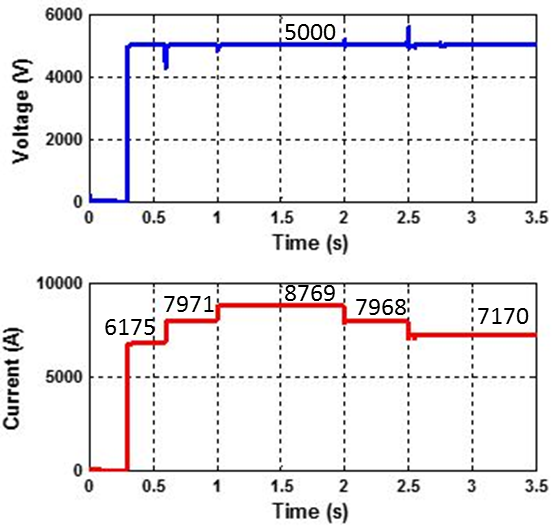
\includegraphics[height=3in, width=3.5in]{f113b}
\end{center}
\caption{Off-line simulation results.}
\label{ch5_f113b}
\end{subfigure}
\begin{subfigure}{1\columnwidth}
\begin{center}
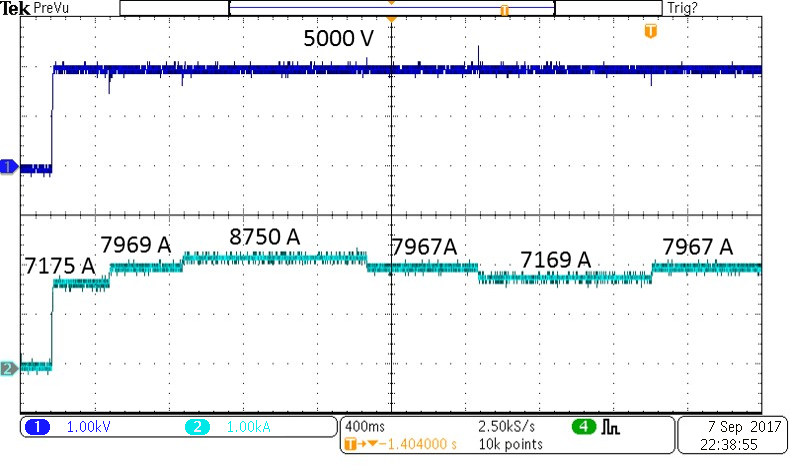
\includegraphics[height=2in, width=3.5in]{f113}
\end{center}
\caption{CHIL results-oscilloscope plots: Ch1: MVDC bus voltage and Ch2: total load current (Ch1: 2.5kV/div, Ch2: 4000A/div).}
\label{ch5_f113a}
\end{subfigure}
\caption{MVDC bus voltage and total load current (case 1).}
\label{ch5_f113}
\end{figure}
%gfhgfhfgjhg
%fghgfhg
\begin{figure}[ht!]
\begin{subfigure}{1\columnwidth}
\begin{center}
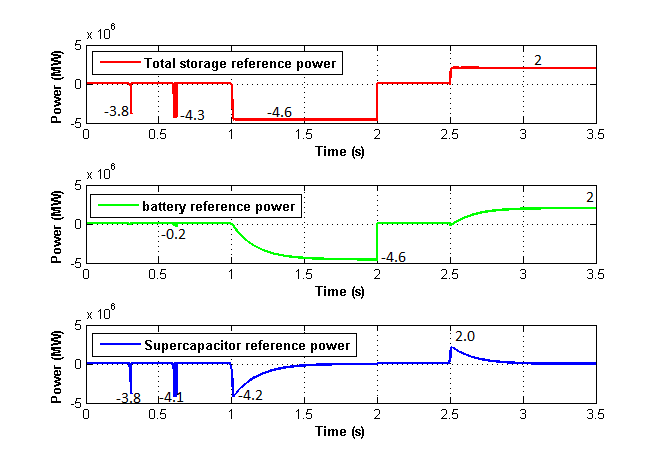
\includegraphics[height=3in, width=3.5in]{f114b}
\end{center}
\caption{Off-line simulation results.}
\label{ch5_f114b}
\end{subfigure}
\begin{subfigure}{1\columnwidth}
\begin{center}
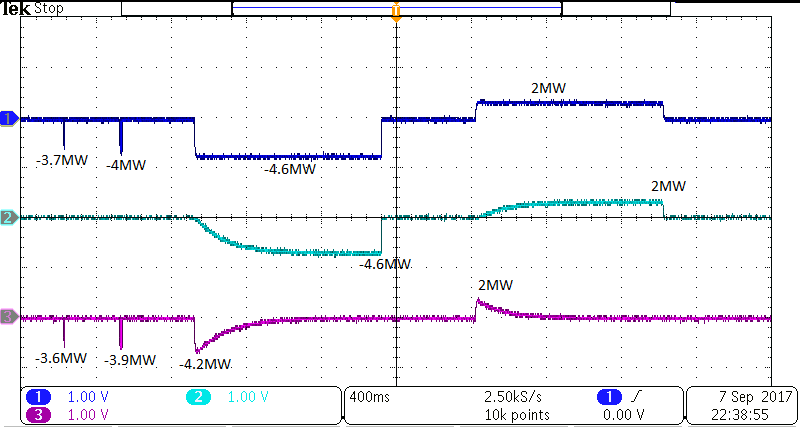
\includegraphics[height=2in, width=3.5in]{f114}
\end{center}
\caption{CHIL results-oscilloscope plots: Ch1: total storage reference power, Ch2: battery reference power, Ch3: supercapacitor reference  power (Ch1, Ch2, Ch3 = 5MW/div).}
\label{ch5_f114a}
\end{subfigure}
\caption{Reference power produced by FL controller and LPF based ESM system (case 1).}
\label{ch5_f114}
\end{figure}
%fdhgfhfgjh
%rfhgfhgfjhgjgh
%gfhgfhfgjhg
%fghgfhg
\begin{figure}[ht!]
\begin{subfigure}{1\columnwidth}
\begin{center}
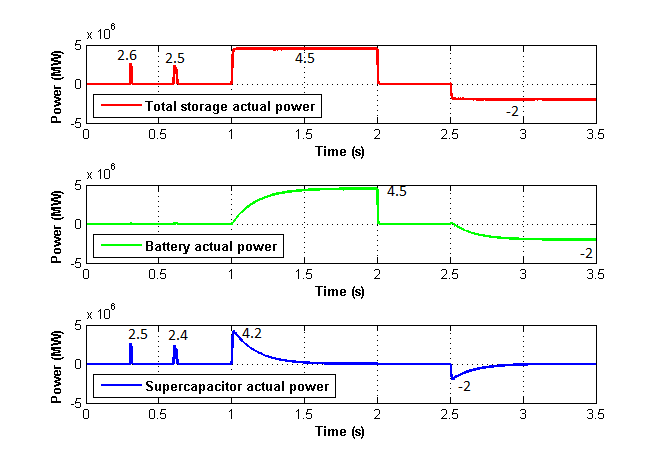
\includegraphics[height=3in, width=3.5in]{f115b}
\end{center}
\caption{Off-line simulation results.}
\label{ch5_f115b}
\end{subfigure}
\begin{subfigure}{1\columnwidth}
\begin{center}
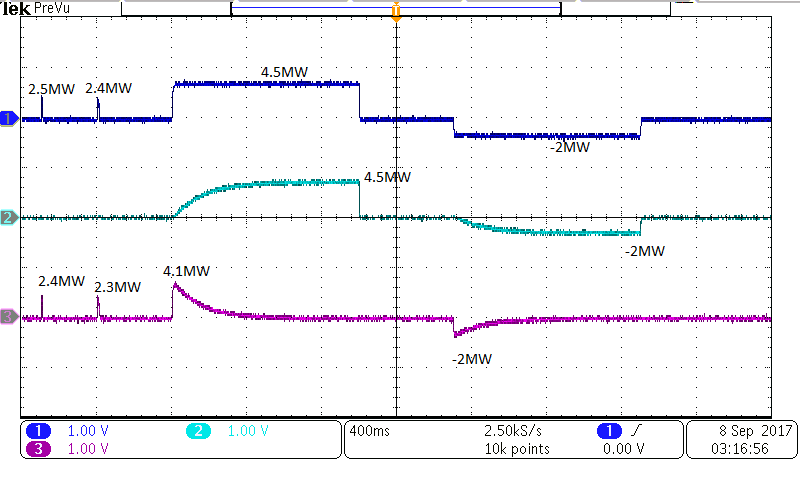
\includegraphics[height=2in, width=3.5in]{f115}
\end{center}
\caption{CHIL results-oscilloscope plots: Ch1: total storage actual power, Ch2: battery actual power, Ch3: supercapacitor actual power (Ch1, Ch2, Ch3 = 5MW/div).}
\label{ch5_f115a}
\end{subfigure}
\caption{Actual power response of the HESS (case 1).}
\label{ch5_f115}
\end{figure}